\chapter{Statistics}
\label{chp:statistics}

Statistics is described as:
\begin{quote}
``Statistics is the discipline that concerns the collection, organization,
analysis, interpretation, and presentation of data.''
\end{quote}


In practice this often means doing some form of analysis to data.
This can be things like taking a mean of a collection of numerical
values and checking if particular relationship exists within the data.
will not consider visualisation of data which is instead covered in
Chapter~\ref{}.



\begin{note}
In this chapter you will cover:
\begin{itemize}
\item 

Calculating measures of central tendency and spread

\item 

Calculating bivariate coefficients

\item 

Fitting a line of best fit

\item 

Using the Normal distribution

\end{itemize}
\end{note}





\section{Tutorial}
\label{\detokenize{tools-for-mathematics/08-statistics/tutorial/main:tutorial}}\label{\detokenize{tools-for-mathematics/08-statistics/tutorial/main::doc}}

You will solve the following problem using a computer to do some of the more
tedious calculations.

Anna is investigating the relationship between exercise and resting heart rate.
She takes a random sample of 19 people in her year group and records for each person
\begin{itemize}
\item 

their resting heart rate, \(h\) beats per minute.

\item 

the number of minutes, \(m\), spent exercising each week.

\end{itemize}


Table~\ref{tab:data_collected_by_anne} shows the data.

\begin{table}[!htbp]
\begin{center}
\begin{tabular}{ll}
\toprule
\(h\) & \(m\)\\
\midrule
76.0 & 5\\
72.0 & 5\\
71.0 & 21\\
74.0 & 30\\
71.0 & 42\\
69.0 & 20\\
68.0 & 20\\
68.0 & 35\\
66 & 80.0\\
64 & 120.0\\
65 & 140.0\\
63 & 180.0\\
63 & 205.0\\
62 & 225.0\\
65 & 237.0\\
63 & 280.0\\
65 & 300.0\\
64 & 356.0\\
64 & 360.0\\
\bottomrule
\end{tabular}
\end{center}
\end{table}



You can see a scatter plot in
Figure~\ref{fig:data_collected_by_anne}.

\begin{figure}[!hbtp]
\begin{center}
\includegraphics[width=.7\textwidth]{./assets/data_collected_by_anne/main.pdf}
\end{center}
\caption{A scatter plot of the data collected by Anne}
\label{fig:data_collected_by_anne}
\end{figure}

\begin{enumerate}

\item 

For all collected values of \(h\) and \(m\) obtain:
\begin{itemize}
\item 

The mean

\item 

The median

\item 

The quartiles

\item 

The standard deviation

\item 

The variation

\item 

The maximum

\item 

The minimum

\end{itemize}

\item 

Obtain the Pearson Coefficient of correlation for the variables \(h\) and \(m\).

\item 

Obtain the line of best fit for variables \(x\) and \(y\) as
defined by:
\begin{equation*}
\begin{split}x=\ln(m)\qquad y=\ln(h)\end{split}
\end{equation*}
\item 

Using the above obtain a relationship between \(m\) and \(h\) of the form:
\begin{equation*}
\begin{split}h=cm^k\end{split}
\end{equation*}
\end{enumerate}



Start by inputting all the data:




\begin{pyin}
h = (
    76.0,
    72.0,
    71.0,
    74.0,
    71.0,
    69.0,
    68.0,
    68.0,
    66.0,
    64.0,
    65.0,
    63.0,
    63.0,
    62.0,
    65.0,
    63.0,
    65.0,
    64.0,
    64.0,
)
m = (
    5,
    5,
    21,
    30,
    42,
    20,
    20,
    35,
    80,
    120,
    140,
    180,
    205,
    225,
    237,
    280,
    300,
    356,
    360,
)
\end{pyin}





The main tool you are going to use for this is \texttt{statistics}.




\begin{pyin}
import statistics as st
\end{pyin}





To calculate the mean:




\begin{pyin}
st.mean(h)
\end{pyin}





\begin{raw}
67.0
\end{raw}







\begin{pyin}
st.mean(m)
\end{pyin}





\begin{raw}
140.05263157894737
\end{raw}





To calculate the median:




\begin{pyin}
st.median(h)
\end{pyin}





\begin{raw}
65.0
\end{raw}







\begin{pyin}
st.median(h)
\end{pyin}





\begin{raw}
120
\end{raw}





To calculate the quartiles, use \texttt{statistics.quantiles} and specify that
you
want to separate the date in to \(n=4\) quarters.




\begin{pyin}
st.quantiles(h, n=4)
\end{pyin}





\begin{raw}
[64.0, 65.0, 71.0]
\end{raw}







\begin{pyin}
st.quantiles(m, n=4)
\end{pyin}





\begin{raw}
[21.0, 120.0, 237.0]
\end{raw}





Note that this calculation confirms the median which corresponds to the 50\%
quartile.
To calculate the sample standard deviation:




\begin{pyin}
st.stdev(h)
\end{pyin}





\begin{raw}
4.123105625617661
\end{raw}







\begin{pyin}
st.stdev(m)
\end{pyin}





\begin{raw}
124.46662813970593
\end{raw}





To calculate the sample variance:




\begin{pyin}
st.variance(h)
\end{pyin}





\begin{raw}
17.0
\end{raw}







\begin{pyin}
st.variance(m)
\end{pyin}





\begin{raw}
15491.941520467837
\end{raw}





To compute that maximum:




\begin{pyin}
max(h)
\end{pyin}





\begin{raw}
76.0
\end{raw}







\begin{pyin}
max(m)
\end{pyin}





\begin{raw}
360
\end{raw}





To compute the minimum:




\begin{pyin}
min(h)
\end{pyin}





\begin{raw}
62.0
\end{raw}







\begin{pyin}
min(m)
\end{pyin}





\begin{raw}
5
\end{raw}





In order to compute the Pearson Coefficient of correlation use
\texttt{statistics.correlation}:




\begin{pyin}
st.correlation(h, m)
\end{pyin}





\begin{raw}
-0.7686142969026402
\end{raw}





This negative value indicates a negative correlation between \(h\) and \(m\),
indicating that the more you exercise the lower your heart rate is likely to be.
To calculate the line of best fit for the transformed variables we need to first
create them. You will do this using a list comprehension. As you are doing
everything numerically, you will use \texttt{math.log} which by default computes the
natural logarithm:




\begin{pyin}
import math
x = [math.log(value) for value in m]
y = [math.log(value) for value in h]
\end{pyin}

Now to compute the line of best fit use \texttt{statistics.linear\_regression}:




\begin{pyin}
slope, intercept = st.linear_regression(x, y)
\end{pyin}

The slope is:

\begin{pyin}
slope
\end{pyin}





\begin{raw}
-0.03854770754231997
\end{raw}





The intercept is:




\begin{pyin}
intercept
\end{pyin}





\begin{raw}
4.368415819445762
\end{raw}





Recall the transformation of the variables:
\begin{equation*}
\begin{split}x=\ln(m)\qquad y=\ln(h)\end{split}
\end{equation*}

You now have the relationship:
\begin{equation*}
\begin{split}y=ax + b\end{split}
\end{equation*}

Where \(a\) corresponds to the \texttt{slope} and \(b\) corresponds to the
\texttt{intercept}.


The question asks for a relationship between \(m\) and \(h\) of the form:
\begin{equation*}
\begin{split}h=cm^k\end{split}
\end{equation*}

You can use \texttt{sympy} to manipulate the expressions:




\begin{pyin}
import sympy as sym

h = sym.Symbol("h")
m = sym.Symbol("m")
a = sym.Symbol("a")
b = sym.Symbol("b")
x = sym.ln(m)
y = sym.ln(h)
\end{pyin}





A general line of best fit for \(x\) and \(y\) can be expressed in terms of \(m\) and
\(h\):




\begin{pyin}
line = sym.Eq(lhs=y, rhs=a * x + b)
line
\end{pyin}




\begin{equation*}
\begin{split}\displaystyle \log{\left(h \right)} = a \log{\left(m \right)} + b\end{split}
\end{equation*}




Taking the exponential of both sides gives the required relationship:




\begin{pyin}
sym.exp(line.lhs)
\end{pyin}




\begin{equation*}
\begin{split}\displaystyle h\end{split}
\end{equation*}






\begin{pyin}
sym.expand(sym.exp(line.rhs))
\end{pyin}




\begin{equation*}
\begin{split}\displaystyle e^{b} e^{a \log{\left(m \right)}}\end{split}
\end{equation*}




Which can be rewritten as:
\begin{equation*}
\begin{split}
e^bm^a
\end{split}
\end{equation*}

Substituting the values for the \texttt{slope} and \texttt{intercept} in to these expressions
gives the required relationship:




\begin{pyin}
sym.exp(line.rhs).subs({a: slope, b: intercept})
\end{pyin}




\begin{equation*}
\begin{split}\displaystyle \frac{78.9185114479915}{m^{0.03854770754232}}\end{split}
\end{equation*}




Figure~\ref{fig:data_collected_by_anne_with_fitted_curve} is a plot that shows
this relationship.







\begin{figure}[!hbtp]
\begin{center}
\includegraphics[width=.7\textwidth]{./assets/data_collected_by_anne_with_fitted_curve/main.pdf}
\end{center}
\caption{A scatter plot of the data collected by Anne with the fitted
relationship.}
\label{fig:data_collected_by_anne_with_fitted_curve}
\end{figure}










\begin{note}
In this tutorial you have
\begin{itemize}
\item 

Calulated values of central tendency and spread

\item 

Calculated some bivariate coefficients

\item 

Fitted a line of best fit

\end{itemize}
\end{note}





\section{How to}
\label{\detokenize{tools-for-mathematics/08-statistics/how/main:how}}\label{\detokenize{tools-for-mathematics/08-statistics/how/main::doc}}

\subsection{Calculate measures of spread and tendency}
\label{\detokenize{tools-for-mathematics/08-statistics/how/main:calculate-measures-of-spread-and-tendency}}

\subsubsection{Calculate a mean}
\label{\detokenize{tools-for-mathematics/08-statistics/how/main:calculate-a-mean}}

You can calculate the mean of a set of data using \texttt{statistics.mean} which takes an
iterable.


\begin{pyin}
statistics.mean(data)
\end{pyin}



For example to calculate the mean of \((1, 5, 10, 12, 13, 20)\):




\begin{pyin}
import statistics as st

data = (1, 5, 10, 12, 13, 20)
st.mean(data)
\end{pyin}





\begin{raw}
10.166666666666666
\end{raw}





\subsubsection{Calculate a median}
\label{\detokenize{tools-for-mathematics/08-statistics/how/main:calculate-a-median}}

You can calculate the median of a set of data using \texttt{statistics.median} which takes an
iterable.


\begin{pyin}
statistics.median(data)
\end{pyin}



For example to calculate the median of \((1, 5, 10, 12, 13, 20)\):




\begin{pyin}
import statistics as st

data = (1, 5, 10, 12, 13, 20)
st.median(data)
\end{pyin}





\begin{raw}
11.0
\end{raw}





\subsubsection{Calculate the population standard deviation}
\label{\detokenize{tools-for-mathematics/08-statistics/how/main:calculate-the-population-standard-deviation}}

You can calculate the population standard deviation of a set of data using \texttt{statistics.pstdev} which takes an
iterable.


\begin{pyin}
statistics.pstdev(data)
\end{pyin}



For example to calculate the population standard deviation of \((1, 5, 10, 12, 13, 20)\):




\begin{pyin}
import statistics as st

data = (1, 5, 10, 12, 13, 20)
st.pstdev(data)
\end{pyin}





\begin{raw}
6.039223643997813
\end{raw}





\subsubsection{Calculate the sample standard deviation}
\label{\detokenize{tools-for-mathematics/08-statistics/how/main:calculate-the-sample-standard-deviation}}

You can calculate the sample standard deviation of a set of data using \texttt{statistics.stdev} which takes an
iterable.


\begin{pyin}
statistics.stdev(data)
\end{pyin}



For example to calculate the sample standard deviation of \((1, 5, 10, 12, 13, 20)\):




\begin{pyin}
import statistics as st

data = (1, 5, 10, 12, 13, 20)
st.stdev(data)
\end{pyin}





\begin{raw}
6.6156380392723015
\end{raw}





\subsubsection{Calculate the population variance}
\label{\detokenize{tools-for-mathematics/08-statistics/how/main:calculate-the-population-variance}}

You can calculate the population variance of a set of data using \texttt{statistics.pvariance} which takes an
iterable.


\begin{pyin}
statistics.pvariance(data)
\end{pyin}



For example to calculate the population variance of \((1, 5, 10, 12, 13, 20)\):




\begin{pyin}
import statistics as st

data = (1, 5, 10, 12, 13, 20)
st.pvariance(data)
\end{pyin}





\begin{raw}
36.47222222222222
\end{raw}





\subsubsection{Calculate the sample variance}
\label{\detokenize{tools-for-mathematics/08-statistics/how/main:calculate-the-sample-variance}}

You can calculate the sample variance of a set of data using \texttt{statistics.variance} which takes an
iterable.


\begin{pyin}
statistics.variance(data)
\end{pyin}



For example to calculate the sample variance of \((1, 5, 10, 12, 13, 20)\):




\begin{pyin}
import statistics as st

data = (1, 5, 10, 12, 13, 20)
st.variance(data)
\end{pyin}





\begin{raw}
43.766666666666666
\end{raw}





\subsubsection{Calculate the maximum}
\label{\detokenize{tools-for-mathematics/08-statistics/how/main:calculate-the-maximum}}

You can calculate the maximum of a set of data use \texttt{max} which takes an iterable:


\begin{pyin}
max(data)
\end{pyin}



For example to calculate the maximum of \((1, 5, 10, 12, 13, 20)\):




\begin{pyin}
data = (1, 5, 10, 12, 13, 20)
max(data)
\end{pyin}





\begin{raw}
20
\end{raw}





\subsubsection{Calculate the minimum}
\label{\detokenize{tools-for-mathematics/08-statistics/how/main:calculate-the-minimum}}

You can calculate the minimum of a set of data use \texttt{max} which takes an iterable:


\begin{pyin}
min(data)
\end{pyin}



For example to calculate the minimum of \((1, 5, 10, 12, 13, 20)\):




\begin{pyin}
data = (1, 5, 10, 12, 13, 20)
min(data)
\end{pyin}





\begin{raw}
1
\end{raw}





\subsubsection{Calculate quantiles}
\label{\detokenize{tools-for-mathematics/08-statistics/how/main:calculate-quantiles}}

To calculate cut points dividing data in to \(n\) intervals of equal probability
you can use \texttt{statistics.quantiles} which takes an iterable and a number of
intervals.


\begin{pyin}
statistics.quantiles(data, n)
\end{pyin}



For example to calculate the cut points that divide \((1, 5, 10, 12, 13, 20)\) in
to 4 intervals of equal probability (in this case the quantiles are called
quartiles):




\begin{pyin}
import statistics as st

data = (1, 5, 10, 12, 13, 20)
st.quantiles(data, n=4)
\end{pyin}





\begin{raw}
[4.0, 11.0, 14.75]
\end{raw}





\subsection{Calculate the sample covariance}
\label{\detokenize{tools-for-mathematics/08-statistics/how/main:calculate-the-sample-covariance}}

To calculate the sample covariance of two data sets you can use
\texttt{statistics.covariance} which takes two iterables.


\begin{pyin}
statistics.covariance(first_data_set, second_data_set)
\end{pyin}



For example to calculate the sample covariance of \(x=(1, 5, 10, 12, 13, 20)\)
and \(y=(3, -3, 6, -2, 1, 2)\):




\begin{pyin}
import statistics as st

x = (1, 5, 10, 12, 13, 20)
y = (3, -3, 6, -2, 1, 2)
st.covariance(x, y)
\end{pyin}





\begin{raw}
1.1666666666666674
\end{raw}





\subsection{Calculate the Pearson correlation coefficient}
\label{\detokenize{tools-for-mathematics/08-statistics/how/main:calculate-the-pearson-correlation-coefficient}}

To calculate the correlation coefficient of two data sets you can use
\texttt{statistics.correlation} which takes two iterables.


\begin{pyin}
statistics.correlation(first_data_set, second_data_set)
\end{pyin}



For example to calculate the correlation coefficient of \(x=(1, 5, 10, 12, 13, 20)\)
and \(y=(3, -3, 6, -2, 1, 2)\):




\begin{pyin}
import statistics as st

x = (1, 5, 10, 12, 13, 20)
y = (3, -3, 6, -2, 1, 2)
st.correlation(x, y)
\end{pyin}





\begin{raw}
0.05325222181462787
\end{raw}





\subsection{Fit a line of best fit}
\label{\detokenize{tools-for-mathematics/08-statistics/how/main:fit-a-line-of-best-fit}}

To carry out linear regression to fit a line of best fit between two data sets
you can use \texttt{statistics.linear\_regression} which takes two iterables and returns
a tuple with the slope and the intercept of the line.


\begin{pyin}
statistics.linear_regression(first_data_set, second_data_set)
\end{pyin}



For example to calculate the correlation coefficient of \(x=(1, 5, 10, 12, 13, 20)\)
and \(y=(-3, -14, -31, -6, -40, -70)\):




\begin{pyin}
import statistics as st

x = (1, 5, 10, 12, 13, 20)
y = (-3, -14, -31, -6, -40, -70)
st.linear_regression(x, y)
\end{pyin}





\begin{raw}
LinearRegression(slope=-3.2338156892612333, intercept=5.543792840822537)
\end{raw}










\begin{figure}[!hbtp]
\begin{center}
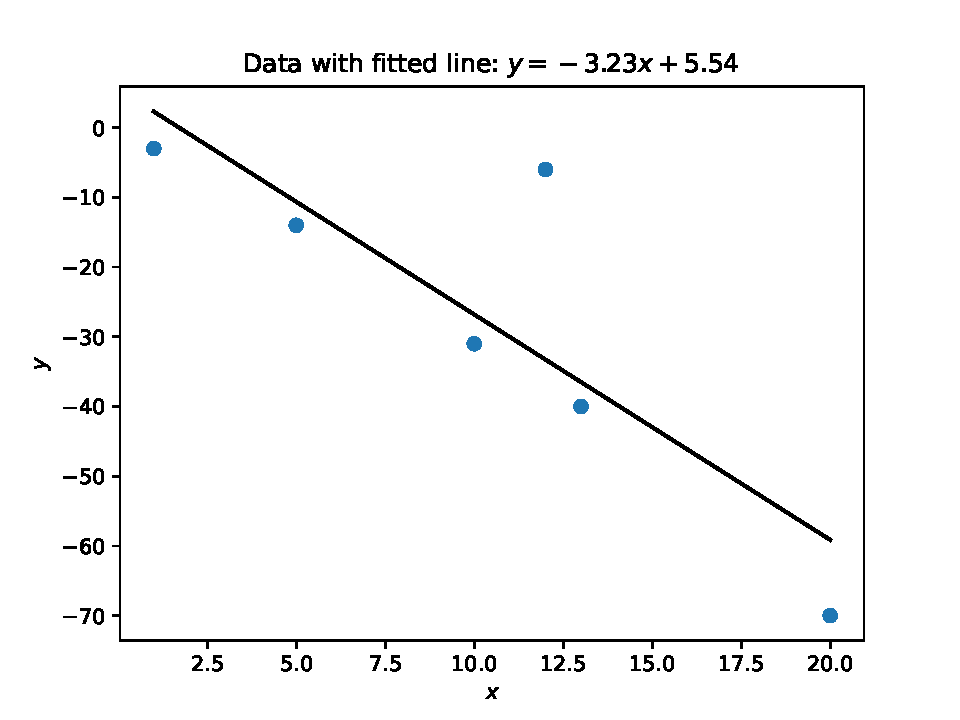
\includegraphics[width=.7\textwidth]{./assets/how_to_fit_a_line/main.pdf}
\end{center}
\caption{A line of best fit.}
\label{fig:how_to_fit_a_line}
\end{figure}







\subsection{How to create an instance of the normal distribution}
\label{\detokenize{tools-for-mathematics/08-statistics/how/main:how-to-create-an-instance-of-the-normal-distribution}}

A normal distribution with mean \(\mu\) and standard deviation \(\sigma\) can be
created using \texttt{statistics.NormalDist}:


\begin{pyin}
statistics.NormalDist(mu, sigma)
\end{pyin}



For example to create the normal distribution with \(\mu=3\) and \(\sigma=.5\):




\begin{pyin}
import statistics as st

distribution = st.NormalDist(mu=3, sigma=.5)
distribution
\end{pyin}





\begin{raw}
NormalDist(mu=3.0, sigma=0.5)
\end{raw}





\subsection{How to use the cumulative distribution function of a normal distribution}
\label{\detokenize{tools-for-mathematics/08-statistics/how/main:how-to-use-the-cumulative-distribution-function-of-a-normal-distribution}}

For an instance of a normal distribution with mean \(\mu\) and \(\sigma\), the
cumulative distribution function which gives \(F(x)=P(X<x)\) (the probability that
the normally distributed random variable is less than \(X\)) can be accessed using
\texttt{statistics.NormaDist.cdf}.


\begin{pyin}
distribution = statistics.NormalDist(mu, sigma)
distribution.cdf(x)
\end{pyin}



For example to find the probability that \(X<2\) for a normally distributed random
variable with \(\mu=3\) and \(\sigma=.5\):




\begin{pyin}
import statistics as st

distribution = st.NormalDist(mu=3, sigma=.5)
distribution.cdf(2)
\end{pyin}





\begin{raw}
0.02275013194817921
\end{raw}





\subsection{How to use the inverse cumulative distribution function of a normal distribution}
\label{\detokenize{tools-for-mathematics/08-statistics/how/main:how-to-use-the-inverse-cumulative-distribution-function-of-a-normal-distribution}}

For an instance of a normal distribution with mean \(\mu\) and \(\sigma\), the
inverse cumulative distribution function which for a given \(p\) gives \(x\) such that \(p=P(X<x)\)
can be accessed using \texttt{statistics.NormaDist.inv\_cdf}.


\begin{pyin}
distribution = statistics.NormalDist(mu, sigma)
distribution.inv_cdf(p)
\end{pyin}



For example to find the value of \(X\) for which a normally distributed random
variable with \(\mu=3\) and \(\sigma=.5\) will be less than with probability \(.7\).




\begin{pyin}
import statistics as st

distribution = st.NormalDist(mu=3, sigma=.5)
distribution.inv_cdf(.7)
\end{pyin}





\begin{raw}
3.2622002563540202
\end{raw}







\section{Exercises}
\label{\detokenize{tools-for-mathematics/08-statistics/exercises/main:exercises}}\label{\detokenize{tools-for-mathematics/08-statistics/exercises/main::doc}}

\begin{enumerate}
\item 

For each of the following sets of data:
\begin{enumerate}

\item Data set 1:
\begin{pyin}
data_set_1 = (
    74,
    -7,
    58,
    82,
    60,
    3,
    49,
    85,
    24,
    99,
    73,
    76,
    11,
    -4,
    61,
    87,
    93,
    13,
    1,
    28,
)
\end{pyin}

\item Data set 2:
\begin{pyin}
data_set_2 = (
    65,
    59,
    81,
    81,
    76,
    93,
    91,
    88,
    55,
    97,
    86,
    94,
    79,
    54,
    63,
    56,
    58,
    77,
    85,
    88,
)
\end{pyin}

\item Data set 3:
\begin{pyin}
data_set_3 = (
    0.31,
    -0.13,
    0.19,
    0.46,
    -0.27,
    -0.06,
    0.20,
    0.42,
    -0.07,
    0.11,
    -0.11,
    -0.43,
    -0.36,
    0.45,
    -0.42,
    0.11,
    0.08,
    0.31,
    0.48,
    0.17,
)
\end{pyin}

\item Data set 4:
\begin{pyin}
data_set_4 = (
    2,
    4,
    2,
    2,
    2,
    2,
    2,
    3,
    2,
    2,
    2,
    4,
    2,
    4,
    2,
    2,
    3,
    4,
    3,
    4,
)
\end{pyin}


Calculate:
\begin{itemize}
\item 

The mean,

\item 

The median,

\item 

The max,

\item 

The min,

\item 

The population standard deviation,

\item 

The sample standard deviation,

\item 

The population variance,

\item 

The sample variance,

\item 

The quartiles (the set of \(n=4\) quantiles),

\item 

The deciles (the set of \(n=10\) quantiles),

\end{itemize}

\end{enumerate}

\item 

Calculate the sample covariance and the correlation coefficient for the
following pairs of data sets from question 1:
\begin{enumerate}

\item 

\texttt{data\_set\_1} and \texttt{data\_set\_4}

\item 

\texttt{data\_set\_3} and \texttt{data\_set\_4}

\item 

\texttt{data\_set\_2} and \texttt{data\_set\_3}

\item 

\texttt{data\_set\_1} and \texttt{data\_set\_2}

\end{enumerate}

\item 

For each of the data sets from question 1 obtain the covariance and
correlation coefficient for the data set with itself.

\item 

Obtain a line of best fit for the pairs of data sets from question 2.

\item 

Given a collection of 250 individuals whose height is normally distributed with
mean 165 and standard deviation 5. What is the expected number of individuals
with height between 150 and 160?

\item 

Consider a class test where the score are normally distributed with mean 65
and standard deviation 5.
\begin{enumerate}

\item 

What is the probability of failing the class test (a score less than 40)?

\item 

What proportion of the class gets a first class mark (a score above 70)?

\item 

What is the mark that only 10\% of the class would expect to get more than?

\end{enumerate}

\end{enumerate}

\section{Further information}
\label{\detokenize{tools-for-mathematics/08-statistics/why/main:further-information}}\label{\detokenize{tools-for-mathematics/08-statistics/why/main::doc}}

\subsection{What is the difference between the sample and the population variance and standard deviation?}
\label{\detokenize{tools-for-mathematics/08-statistics/why/main:what-is-the-difference-between-the-sample-and-the-population-variance-and-standard-deviation}}

For a given set of \(N\) values \(x_1, x_2, \dots, x_N\) with mean \(\bar x\) the sample
standard deviation is given by:
\begin{equation*}
\begin{split}
\sigma = \sqrt{\frac{\sum_{i=1}^N{(x_i - \bar x) ^ 2}}{N - 1}}
\end{split}
\end{equation*}

The sample variance is given by:
\begin{equation*}
\begin{split}
\sigma ^ 2
\end{split}
\end{equation*}

The population standard deviation is given by:
\begin{equation*}
\begin{split}
\sigma = \sqrt{\frac{\sum_{i=1}^N{(x_i - \bar x) ^ 2}}{N}}
\end{split}
\end{equation*}

The population variance is given by:
\begin{equation*}
\begin{split}
\sigma ^ 2
\end{split}
\end{equation*}

The population standard deviation and/or variance should be used when the data set in question
is for the entire population.


The sample standard deviation and/or variance should be used when the data set in question is a
sample of the entire population. The modification in the calculation is to
counteract a potential bias.


\subsection{How to plot a line of best fit?}
\label{\detokenize{tools-for-mathematics/08-statistics/why/main:how-do-we-plot-a-line-of-best-fit}}

The main library for plotting is called \texttt{matplotlib} and
Chapter~\ref{} covers this library in more detail.


However below is some code to plot the data and regression line for two
collections of data. Figure~\ref{fig:example_plot_of_fitted_line} gives the output.

\begin{pyin}
import statistics as stat
import matplotlib.pyplot as plt

x = (0, 2, 2, 3, 4, 5.6)
y = (-1, -3, -4, -5, 4, -7)

slope, intercept = stat.linear_regression(x, y)

start_point, end_point = min(x), max(x)
image_start_point = slope * start_point + intercept
image_end_point = slope * end_point + intercept

plt.figure()
plt.scatter(x, y)
plt.plot((start_point, end_point), (image_start_point, image_end_point))
plt.xlabel("$x$")
plt.ylabel("$y$")
\end{pyin}


\begin{figure}[!hbtp]
\begin{center}
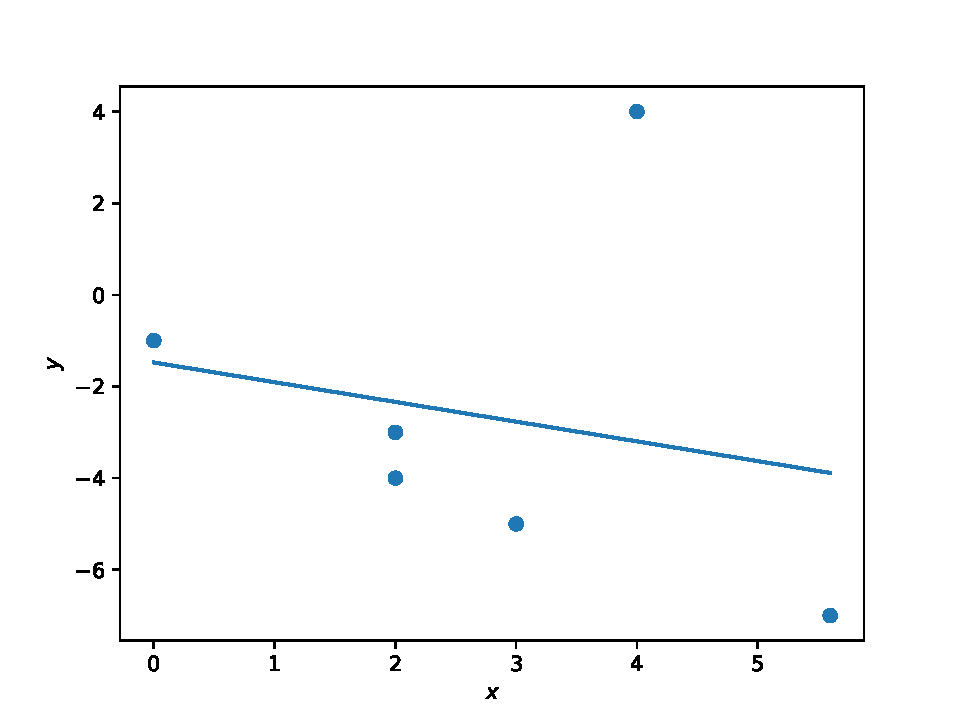
\includegraphics[width=.7\textwidth]{./assets/example_plot_of_fitted_line/main.pdf}
\end{center}
\caption{Example of plotting a fitted line}
\label{fig:example_plot_of_fitted_line}
\end{figure}



\subsection{What other statistics tools exist in Python?}
\label{\detokenize{tools-for-mathematics/08-statistics/why/main:what-other-statistics-tools-exist-in-python}}

The \texttt{statsmodels} library allows for a wider breadth of statistical
analysis.
The \texttt{scikit-learn} library is arguably one of the most popular python libraries.
It is technically a library for machine learning and not statistics.


\subsection{What is the difference between machine learning and statistics}
\label{\detokenize{tools-for-mathematics/08-statistics/why/main:what-is-the-difference-between-machine-learning-and-statistics}}

In a lot of cases the difference here is more question of vocabulary than
actual tangible differences.


For example the \texttt{scikit-learn} library has a tool for linear regression as does
the \texttt{statsmodels} and the \texttt{statistics} library.


In practice statistics is often more descriptive, for example using linear
regression to understand the relationship between two variables. Whereas machine
learning is more predictive, for example using liner regression to predict one
variable value from another.


A lot of modern applied mathematics using tools such as neural networks which
are usually discussed as tools from the machine learning.
